\renewcommand{\appendixpagename}{\vspace*{\fill}\centering \textit{Web Appendix:} Defining and emulating target trials of the effects of postexposure vaccination using observational data\vspace*{\fill} } % Appendices title

\begin{appendices}

    \renewcommand{\thefigure}{A\arabic{figure}}
    \setcounter{figure}{0}
    
    \renewcommand{\thetable}{A\arabic{table}}
    \setcounter{table}{0}
    
    \renewcommand{\theequation}{A\arabic{equation}}
    \setcounter{equation}{0}

    \newpage

    \section{Appendix}
    \begin{refsection}  
    \subsection{Day zero randomization designs} \label{sec:dayzero}
    In the main text, we discussed two trial designs starting on postexposure day zero. In the first, participants are enrolled on postexposure day zero, randomized, and immediately receive either vaccine or no vaccine with the goal of estimating the $\Delta$-day vaccine effectiveness in the ideal case in which there is no delay between exposure and vaccination. Under perfect adherence this trial targets the estimand
    $$VE(0) = 1 - \dfrac{\Pr[Y^{x = 0} = 1]}{\Pr[Y^{x > \Delta} = 1]}$$
    or, alternatively,
    $$VE(0) = 1 - \dfrac{\Pr[Y^{\overline{a}_{K} = 1} = 1]}{\Pr[Y^{\overline{a}_{K} = 0} = 1]}$$
    using our definition of time-varying treatment $A_t$ with $K = \Delta - 1$ and overbars representing past history, i.e. $\overline{A}_k = (A_0, A_1, \ldots, A_k)$. This value is likely an upper bound on vaccine effectiveness under more plausible scenarios of delay.

    In the second design, participants are still enrolled and randomized on postexposure day zero, but they are then further randomly assigned a postexposure date to receive the vaccine.  Under perfect adherence, the casual contrast of interest is now the $t$-specific vaccine effectiveness
    $$VE(t) = 1 - \frac{\Pr[Y^{x = t} = 1]}{\Pr[Y^{x > \Delta} = 1]}.$$
    or, alternatively,
    $$VE(t) = 1 - \dfrac{\Pr[Y^{(\overline{a}_{t-1}=0, \underline{a}_{t} = 1)} = 1]}{\Pr[Y^{\overline{a}_{K} = 0} = 1]}$$
    with underbars representing future history, i.e. $\underline{A}_k = (A_k, A_{k+1}, \ldots, A_{\Delta - 1})$. This could be used, for instance, to determine the time window public health officials and policymakers should advise individuals at risk of exposure to seek vaccination within if they are exposed (see Section \ref{sec:maxdelay}).
    \clearpage
    \subsection{Fixed enrollment period designs} \label{sec:enrollment}

    Also mentioned in the main text, when the timing of vaccination is not under the strict control of the investigator, a possible design is to specify a fixed time window in which participants are eligible to be vaccinated and randomize them on the postexposure day they present. Under perfect adherence, this design could then target the $t$-specific vaccine effectiveness among those presenting symptom-free, i.e.
    $$
    VE_{T > t}(t) = 1 - \frac{\Pr[Y^{x = t} = 1 \mid X \geq t, T > t]}{\Pr[Y^{x > \Delta} = 1 \mid X \geq t, T > t]}
    $$
    or 
    $$VE_{T > t}(t) = 1 - \dfrac{\Pr[Y^{(\overline{A}_{t-1}, \underline{1}_{t})} = 1\mid \overline{A}_{t-1} = 0, T > t]}{\Pr[Y^{(\overline{A}_{t-1}, \underline{0}_{t})} = 1\mid \overline{A}_{t-1} = 0, T > t]}$$
    by comparing vaccine and no vaccine groups within enrollment strata. Note that, in general, the $t$-specific vaccine efficacies, $VE_{T > t}(t)$, targeted in this trial will not be the same as the $VE(t)$ defined previously as they are conditional on presentation time and being symptom-free at enrollment. More often, in practice, the $t$-specific estimates $VE_{T > t}(t)$ are pooled together into a weighted average effectiveness over the enrollment period. However, we stress caution in interpreting pooled estimates. Because participants are allowed to present naturally rather than being assigned a time at day zero, those that present earlier may be systematically different than those presenting later with respect to their risk of developing clinical disease. Therefore the pooled estimates are among a subpopulation who survive symptom-free and may not generalize to other populations with different propensities for delay. 
    \clearpage 
    \subsection{Adding a grace period} \label{sec:graceperiod}

    An alternative to the day zero design which also allows for delays in vaccination but doesn't require consideration of all possible delay regimes is to specify a \textit{grace period}, i.e. a fixed time window after randomization in which vaccination can be initiated. For example, in a postexposure trial of a varicella vaccine, investigators might randomize sibling contacts of an index case to vaccine or placebo and then specify contacts are adherent if they receive their assigned treatment within \textit{within 72 hours} of the appearance of the first skin lesion in the index case. Under this design, the causal target would be the average vaccine effectiveness if received during the $m$ days of the grace period, i.e.
    $$
    \overline{VE}_m = 1 - \frac{\Pr[Y^{g(X,m)} = 1]}{\Pr[Y^{x > \Delta} = 1]}
    $$ 
    where
    \begin{gather*}
        g(X,m): \text{get vaccinated within $m$ days of exposure under the expected vaccine } \\ \text{ administration pattern }  f^*(X \mid \overline{L}_t, X > t, T > t)
    \end{gather*}
    and where, for instance, in the hypothetical varicella trial $m = 3$. Although in theory randomization could occur on any postexposure day followed by $m$-day grace period, in practice grace periods starting from randomization on day zero probably make the most sense. When effectiveness varies by the time since exposure, as it most certainly does for postexposure vaccines, a grace period design estimates the average effectiveness \textit{under the ``natural'' course of vaccination over the grace period}, i.e.
     $$f^*(X \mid \overline{L}_t, X > t, T > t) = \begin{cases} 
        f^{obs}(X \mid \overline{L}_t, X > t, T > t) & : t < m\\
        1 & : t \geq m
     \end{cases},$$
    or alternatively
    $$f^*(A \mid \overline{L}_t, \overline{A}_{t-1}, D_{t-1} = 0) = \begin{cases} 
        f^{obs}(A \mid \overline{L}_t, \overline{A}_{t-1}, D_{t-1} = 0) & : t < m\\
        1 & : t \geq m
     \end{cases}$$
    using time-varying treatment $A_t$ instead of $X$ and time-varying disease indicator $D_k$ in place of $T$. We note the effectiveness under other stochastic strategies may be possible under additional assumptions \cite{wanis_role_2022}. This implies that two trials identical in all respects except for the distribution of vaccinations over the grace period could yield substantially different estimates. Therefore, a trialist pursuing this design has to strike a balance when defining a grace period between ensuring the period is short enough that benefit is immunologically possible and the trial is adequately powered, but also long enough that the regime is clinically feasible under reasonable assumptions about how quickly patients are notified of their exposure to a case and can access a vaccine in the real world. If properly conceived, a grace period design can provide evidence about average effectiveness of postexposure vaccination administered within a certain window under real world conditions. As such it may be a more useful estimate for population planning or modeling studies than those produced by the fixed enrollment period design above. 
    
    %When there's no effect modification by covariates, the average effectiveness is equal to $VE(t)$ standardized over the distribution of vaccine administration times during the grace period, i.e.
    %$$\overline{VE}_\delta = \sum_{t = 1}^\delta VE(t) \times f^*_X(t \mid \overline{L}_t, X > t, T > t).$$
    \clearpage
    \subsection{Example target trial specification for JYNNEOS vaccine}\label{sec:trial_spec}
    \subsubsection*{Eligibility}

    Individuals over 18 years of age who had an intermediate or high risk exposure to a person with laboratory confirmed mpox case, no history of JYNNEOS vaccination, no positive PCR for mpox or other orthopox virus at enrollment, and who were referred within 14 days of exposure are eligible for this study. We use the CDC definitions of high and intermediate risk exposures \cite{cdc_mpox_2022} for mpox (Table \ref{tab:protocol}).

    \subsubsection*{Treatment strategies}
    1) a single JYNNEOS vaccination dose (either the intradermal or subcutaneous regimen) at enrollment and 2) no mpox vaccination dose over the 21-day follow up period. 

    \subsubsection*{Assignment procedures}
    Individuals are randomly assigned to one strategy within permuted assignment blocks defined by day of presentation at the clinic and possibly other covariates of interest. Individuals are aware of the strategy to which they have been assigned (unblinded).
    
    \subsubsection*{Outcomes}
    The primary outcome is PCR-confirmed mpox or orthopox infection within 21 days of exposure. Secondary outcomes could include disease severity or safety endpoints. 

    \subsubsection*{Follow-up period}
    Follow-up begins at date of exposure to the index case and ends at either the occurrence of the outcome, 21 days after exposure, or loss to follow-up, whichever occurs first (We discuss the possibility of delayed outcomes based on biology and their implications for observational emulations in Appendix section \ref{sec:delayed_followup}).

    \subsubsection*{Causal contrasts}
    Intent-to-treat and per protocol effects of JYNNEOS vaccination.

    \subsubsection*{Statistical analysis}
    In the intention-to-treat (ITT) analysis, we compare the cumulative incidences in each group defined by assignment and calculate the vaccine effectiveness as $VE = 1 - \frac{\Pr[Y = 1 \mid Z = 1]}{\Pr[Y = 1 \mid Z = 0]}$ where $Z$ is an indicator of random assignment to strategy (1) or (2). In the stratified design, we can either calculate ITT effects for the $t$-specific vaccine efficacies separately or, under additional assumptions, pool together into a 14-day average. Cumulative incidence curves can be estimated in each arm via the Kaplan-Meier estimator or a pooled logistic model. Loss to follow-up can bias estimates of ITT effects \cite{stensrud_why_2020}. We can adjust for the resulting selection bias under the assumption that measured covariates (in practice often just baseline) include all determinants of loss to follow-up and the outcome.

    The per-protocol analysis is similar to the ITT analysis except that individuals are censored if they deviate from their assigned treatment strategy, e.g. by declining the vaccine when assigned to vaccine or obtaining it outside of the trial if assigned to no vaccine. We can adjust for the possible time-varying selection bias due to censoring for protocol deviations (and/or loss to follow-up) through an appropriate g-method under the assumption that the measured variables include approximately all determinants of adherence and the outcome. 95\% confidence intervals may be estimated via bootstrapping.

    \clearpage
    \subsection{Identifiability conditions}\label{sec:identifiability}
    Here, we review the conditions under which data from an observational emulation can be used to identify the causal contrasts of interest in the target trial designs discussed above. As previously, let $D^g_{k+1}$, $A^g_{k+1}$, and $L^g_{k+1}$ represent the counterfactual outcome, vaccination, and covariate history under vaccination strategy $g$. To identify effects, the following conditions must hold for $k = 0, \ldots, \Delta - 1$: 
    \begin{enumerate}
        \item \textit{Consistency:} If $\overline{A}_k = \overline{a}_k^g$ then $D_{k+1} = D^g_{k+1}$ and $\overline{L}_{k} = \overline{L}^g_{k}$
        \item \textit{Sequential exchangeability:} $D^g_{k+1} \perp \!\!\! \perp A^g_k \mid \overline{L}_k = \overline{l}_k, \overline{A}^g_{k-1} = \overline{a}_{k-1}^g, D_k = 0$
        \item \textit{Positivity:} $f_{\overline{L}_k,\overline{A}^g_{k-1},D_k}(\overline{l}_k, \overline{a}_{k-1}^g, 0) \neq 0 \implies \Pr(A_k = a^g_k \mid \overline{L}_k = \overline{l}_k, \overline{A}_{k -1} = \overline{a}^g_{k-1}) > 0$ 
    \end{enumerate}
    The first condition requires that our vaccination strategies are sufficiently well-defined such that they match an intervention that would be assigned in the target postexposure trial and are reflected in the observed vaccination patterns in our observational study. The second condition is alternatively known as the ``no unmeasured confounding assumption'' and requires that sufficient covariate information is collected in the observational study such that potential outcomes are as if randomized, i.e. conditionally independent, given past vaccination and covariate history. The final assumption requires that there is a positive probability of receiving a vaccine in each covariate strata.

    In Figure \ref{fig:swig1}, we use Single World Intervention Graphs (SWIGs) to represent the postexposure process, i.e. time-varying evolution of vaccination, symptoms, and covariates. Because SWIGs explicitly depict potential outcomes under interventions they are well-suited to reasoning about exchangeability conditions. On a SWIG, a potential outcome $D^g_t$ is conditionally independent of treatment $A_t$ if there are no unblocked \textit{backdoor} paths connecting $D^g_t$ and $A_t$ conditional on past treatment and covariate history. Using SWIGs helps us illuminate a subtle point regarding the conditional exchangeability assumption under the grace period strategy compared to the static strategies in the fixed enrollment period and day zero designs, which is developed further in \cite{wanis_role_2022}. Specifically, when there is an unmeasured common cause of vaccination $U_A$ at any two time-points exchangeability will hold for the static regimes of the fixed-enrollment and day zero designs, but it will not hold for the grace period under natural initiation of treatment. 

    \begin{figure}[p]
        \centering
        \begin{subfigure}{\linewidth}
            \centering
            \begin{tikzpicture}[> = stealth, shorten > = 1pt, auto, node distance = 2.25cm, inner sep = 0pt,minimum size = 0.5pt, semithick]
                \tikzstyle{every state}=[
                  draw = white,
                  fill = white
                ]
                \node[state] (l0) {$L_0$};
                \node[state] (a0) [right of=l0] {$A_0 \mid \textcolor{red}{a_0}$};
                \node[state] (y1) [right of=a0] {$D^{\textcolor{red}{a_0}}$};
                \node[state] (l1) [right of=y1] {$L^{\textcolor{red}{a_0}}$};
                \node[state] (a1) [right of=l1] {$A^{\textcolor{red}{a_0}} \mid \textcolor{red}{a_1}$};
                \node[state] (y2) [right of=a1] {$D_2^{\textcolor{red}{a_0, a_1}}$};
                \node[state] (u0) [below of=y1] {$U_L$};
                \node[state] (u1) [below of=l0] {$U_A$};

                \path[->] (l0) edge node {} (a0);
                \path[->] (l0) edge [out=20, in=160, looseness=1.5] node {} (l1);
                \path[->] (l0) edge [out=20, in=160, looseness=1.5] node {} (a1);
                \path[->] (l0) edge [out=20, in=160, looseness=1.5] node {} (y2);
            
                \path[->] (a0) edge  node {} (y1);
                \path[->] (a0) edge [out=20, in=160, looseness=1.5] node {} (l1);
                \path[->] (a0) edge [out=20, in=160, looseness=1.5] node {} (a1);
                \path[->] (a0) edge [out=20, in=160, looseness=1.5] node {} (y2);
                    
                \path[->] (y1) edge  node {} (l1);
                \path[->] (y1) edge [out=20, in=160, looseness=1.5] node {} (a1);
                \path[->] (y1) edge [out=20, in=160, looseness=1.5] node {} (y2);
        
                \path[->] (l1) edge node {} (a1);
                \path[->] (l1) edge [out=20, in=160, looseness=1.5] node {} (y2);
                
                \path[->] (a1) edge node {} (y2);
                
                \path[->] (u0) edge node {} (y1);
                \path[->] (u0) edge node {} (y2);
                \path[->] (u0) edge node {} (l0);
                \path[->] (u0) edge node {} (l1);

                \path[->] (u1) edge node {} (a0);
                \path[->] (u1) edge node {} (a1);
                \end{tikzpicture}
                \caption{SWIG for static regime in fixed-enrollment period and day zero designs.}
        \end{subfigure}
        \begin{subfigure}{\linewidth}
            \centering
        \begin{tikzpicture}[> = stealth, shorten > = 1pt, auto, node distance = 2.25cm, inner sep = 0pt,minimum size = 0.5pt, semithick]
        \tikzstyle{every state}=[
          draw = white,
          fill = white
        ]
        \tikzset{longstate/.style={ellipse,
        draw = white,
        fill = white}}
        \node[state] (l0) {$L_0$};
        \node[longstate] (a0) [right of=l0] {$A_0 \mid A_0^{\textcolor{red}{g+}}$};
        \node[state] (y1) [right of=a0] {$D^{\textcolor{red}{g}}_1$};
        \node[state] (l1) [right of=y1] {$L^{\textcolor{red}{g}}_1$};
        \node[longstate] (a1) [right of=l1] {$A^{\textcolor{red}{g}}_1 \mid A_1^{\textcolor{red}{g+}}$};
        \node[state] (y2) [right of=a1] {$D_2^{\textcolor{red}{g}}$};
        \node[state] (u0) [below of=y1] {$U_L$};
        \node[state] (u1) [below of=l0] {$U_A$};

        \path[->] (l0) edge node {} (a0);
        \path[->] (l0) edge [out=20, in=160, looseness=1.5] node {} (l1);
        \path[->] (l0) edge [out=20, in=160, looseness=1.5] node {} (a1);
        \path[->] (l0) edge [out=20, in=160, looseness=1.5] node {} (y2);
    
        \path[->] (a0) edge  node {} (y1);
        \path[->] (a0) edge [out=210, in=330, looseness=2, dashed] node {} (a0);
        \path[->] (a0) edge [out=20, in=160, looseness=1.5] node {} (l1);
        \path[->] (a0) edge [out=20, in=160, looseness=1.5] node {} (a1);
        \path[->] (a0) edge [out=20, in=160, looseness=1.5] node {} (y2);
            
        \path[->] (y1) edge  node {} (l1);
        \path[->] (y1) edge [out=20, in=160, looseness=1.5] node {} (a1);
        \path[->] (y1) edge [out=20, in=160, looseness=1.5] node {} (y2);

        \path[->] (l1) edge node {} (a1);
        \path[->] (l1) edge [out=20, in=160, looseness=1.5] node {} (y2);
        
        \path[->] (a1) edge [draw=cyan] node {} (y2);
        \path[->] (a1) edge [out=210, in=330, looseness=2, draw=cyan, dashed] node {} (a1);

        \path[->] (u0) edge node {} (y1);
        \path[->] (u0) edge [out=0, in=220] node {} (y2);
        \path[->] (u0) edge node {} (l0);
        \path[->] (u0) edge node {} (l1);

        \path[->] (u1) edge [draw=cyan] node {} (a0);
        \path[->] (u1) edge [draw=cyan] node {} (a1);
        \end{tikzpicture}
        \caption{SWIG for natural regime in grace period design.}
        \end{subfigure}
        \caption{Causal graphs depicting the postexposure process under different interventions. The variables $L_0$, $L_1$, $A_0$, $A_1$, $D_1$, and $D_2$ are as defined in the main text. Unmeasured variable $U_L$ is a common cause of measured covariates and the outcome (symptoms) and unmeasured variable $U_A$ is a common cause of vaccination. The blue line highlights the open backdoor path which leads to a failure of the sequential exchangeability assumption.        \label{fig:swig1}
        }

    \end{figure}

    \clearpage

    
    \subsection{Data setup and additional emulation details} \label{sec:datamanip}
    Here, we demonstrate the data manipulation steps required to emulate the three trial designs ---day zero, fixed enrollment period, and grace period--- discussed above using observational data. Our goal is to emulate the analysis that would have been conducted in the ideal trial assuming that the necessary identifiability conditions are valid in the observational study.

    Two crucial differences between a randomized trial and an observational study are that 1) the former has a well defined start of follow up, or \textit{time zero}, from which study outcomes are assessed and 2) all participants are assigned a particular treatment strategy. By contrast observational studies generally do not have a uniquely defined time zero and participants may have data consistent with multiple treatment strategies. In each design, certain data manipulation steps are applied to the observational data to solve these issues. 

    \subsubsection{Fixed enrollment period trial emulation}\label{sec:fixed_emulation}
    When emulating a fixed enrollment period design, the issue is that participants in the observational data generally meet the eligibility criteria at multiple time points, and therefore there is no unambiguous time zero from which to start follow up. For instance, consider a postexposure vaccination trial in which participants are eligible anytime in the first 5 days after exposure if they have no previous vaccination history and no symptoms at presentation. In a real trial the participant would be enrolled and randomized on a particular day and that would be their time zero. In the observational data, a participant may meet these criteria continuously, for instance between days 0 and 4. The question is then when should their follow-up start? On day 0, 1, 2, 3, or 4? The choice has to be applied equivalently to vaccinated and unvaccinated participants to avoid \textit{immortal time bias}. One possibility is to randomly choose a start time among the days they are eligible. However, a more efficient choice is to use every eligible time by emulating a sequence of multiple nested target trials each with a different start time. A natural choice for postexposure vaccination for a pathogen with a relatively short incubation period is to emulate a series of daily nested trials, i.e. on day zero condition on those who meet the eligibility criteria and compare those who are vaccinated on that day to those who are unvaccinated on that day, and then repeat on all days within the fixed enrollment period (schematic Figure \ref{fig:design1}). Participants in the observational study can be enrolled in trials starting on multiple days as long as they meet the eligibility criteria at time zero. As suggested in \cite{guo_discussion_2021-1}, this design is akin to estimating the parameters of the structural nested model
    \begin{equation*}
        \beta_{t, \Delta}(\overline{V}_t) = \log \frac{\Pr[D_t^{(\overline{A}_{t-1}, 1, \underline{1}_{t+1})}  = 1| I_t = 1, \overline{V}_t, D_{t-1} = 0]}{\Pr[D_t^{(\overline{A}_{t-1}, 0, \underline{0}_{t+1})} = 1 |  I_t = 1, \overline{V}_t, D_{t-1} = 0]}
    \end{equation*}
    where $I_t$ is an indicator that a participant is eligible for the trial starting on day $t$ and $V_t$ are a subset of covariates which may be effect modifiers.

    To demonstrate the required data manipulation steps, consider the six individuals shown in Table \ref{tab:example1} with vaccination and symptom onset times recorded during a hypothetical observational study. To emulate a trial with a fixed five day enrollment period postexposure, we create one copy of the dataset for each trial day. Then in each copy we apply the proper eligibility criteria (e.g. individuals should be disease-free and not vaccinated on a previous day) and assign those vaccinated on that trial day to be ``vaccinated'' and those who have not been vaccinated yet to be ``unvaccinated''. For example, individual 2 in Table \ref{tab:example1} is vaccinated on on day 2 and doesn't develop symptoms, therefore in the emulation they will participate in 3 trials (i.e. those starting on postexposure day 0, 1, and 2). In trials starting after postexposure day 2 they are no longer eligible because they have already been vaccinated. In each trial, follow up time is adjusted to start on the postexposure day of interest and end either at symptom onset or at the maximum follow up day which may be fixed from the index exposure day or be of fixed length from the trial day. In intention-to-treat analyses, participants are ``assigned'' based on their baseline status in the nested trial and followed throughout regardless of whether they later deviate. In per protocol analyses, individuals in each nested trial are censored when they deviate from their baseline assignment in that trial. For example, individual 3 in Table \ref{tab:example1} is unvaccinated in trials starting on days 0 through 3, but in each of these trials is censored on day 4 in the per protocol analysis because they deviate from their baseline assignment by becoming vaccinated.
    
    \begin{table}[t]
        \small
        \centering
        \caption{Enrollment of six hypothetical individuals in daily nested trials for 5-day vaccination window based on observed data.\label{tab:example1}}
        \begin{tabular}{cC{0.9in}C{0.9in}C{1in}C{1in}C{0.9in}C{0.9in}}
        \toprule
        \makecell[c]{ID} & \makecell[c]{Vaccination \\ (1: yes, 0: no)} & \makecell[c]{Day of \\ vaccination} & \makecell[c]{Clinical disease \\ (1: yes, 0: no)} & \makecell[c]{Day of \\ disease onset} & \makecell[c]{No. of trials \\ enrolled} \\
        \midrule
            1 & 1 & 0 & 0 & - & 1 (day 0) \\
            2 & 1 & 2 & 0 & - & 3 (days 0-2) \\
            3 & 1 & 4 & 1 & 8 & 5 (days 0-4) \\
            4 & 1 & 7 & 1 & 2 & 2 (days 0-1) \\
            5 & 0 & - & 0 & - & 6 (days 0-5) \\
            6 & 0 & - & 1 & 5 & 5 (days 0-4) \\
        \bottomrule
        \end{tabular}
    \end{table}

    
    \subsubsection{Day zero trial emulation}\label{sec:dayzero_emulation}

    When emulating a day zero trial in which participants are randomized to a particular delay before receiving a vaccine after exposure, the issue is that participants in the observational data will have data consistent with multiple delay regimes. Consider a trial where participants are randomized on day zero to one of the following strategies: (1) receive vaccine on day zero, (2) receive vaccine on day one, (3) receive vaccine on day two, (4) receive vaccine on day three, or (5) to receive no vaccine over the follow up period (schematic Figure \ref{fig:design2}). In a real trial participants would be assigned to one of the five regimes at the start. In the observational data, however, some individuals will get vaccinated on day 0 and therefore only have data compatible with the first strategy, but others will not get vaccinated on day zero and will have data compatible with multiple strategies at baseline. The question is now which strategy should we assign them to? As with the start time in the previous design, one option is to pick a single strategy at random from the strategies their data is consistent with. However, the more efficient choice is to assign them to all possible strategies by creating exact copies ---often called clones--- of any individual whose data is consistent with multiple regimes and assign each of their clones to a different strategy. 

    To demonstrate the required data manipulation steps, let's return to the six hypothetical individuals from Table \ref{tab:example1}, but now in Table \ref{tab:example2} we will use their data to emulate a day zero trial in which participants are randomized to strategies (1)-(5) in previous paragraph. Starting with the first individual, they are vaccinated on day zero and therefore have data consistent only with strategy (1), thus they are not cloned. The second individual, however, is not vaccinated until day 2 and therefore at time zero they have data consistent with any of the strategies (1)-(5), thus we make five clones of the second individual by copying their data five times and assigning each observation to a different regime. We then follow each clone forward and censor them when they deviate from their assigned regime. For instance, we know the second individual is vaccinated on day 2, therefore on day 0 we censor the clone assigned to strategy (1) because they were not vaccinated on that day. Likewise, on day 1 we censor the clone assigned to strategy (2) because they were not vaccinated on that day either, then on day 2 we censor all the remaining clones except the one assigned to strategy (3). Importantly, if the individual has symptoms before a clone is censored, as is the case for the strategy (3) and (4) clones for individual 4, then all clones will have symptoms and therefore the case is assigned to all strategies. This multiple allocation of events prevents the bias that could arise if events occurring during the delay period are systematically assigned to one of the five strategies only.

    \begin{table}[t]
        \small
        \centering
        \caption{Emulation of day zero trial with five vaccination delay strategies using data from six hypothetical individuals.\label{tab:example2}}
        \begin{tabular}{cC{0.9in}C{0.9in}C{1in}C{1in}C{1.1in}}
        \toprule
        \makecell[c]{ID} & \makecell[c]{Vaccination \\ (1: yes, 0: no)} & \makecell[c]{Day of \\ vaccination} & \makecell[c]{Clinical disease \\ (1: yes, 0: no)} & \makecell[c]{Day of \\ disease onset} & \makecell[c]{No. of clones \\ (regimes)} \\
        \midrule
            1 & 1 & 0 & 0 & - & 1 (1) \\
            2 & 1 & 2 & 0 & - & 5 (1-5) \\
            3 & 1 & 4 & 1 & 8 & 5 (1-5) \\
            4 & 1 & 7 & 1 & 2 & 5 (1-5) \\
            5 & 0 & - & 0 & - & 5 (1-5) \\
            6 & 0 & - & 1 & 5 & 5 (1-5) \\
        \bottomrule
        \end{tabular}
    \end{table}

    \subsubsection{Grace period trial emulation}\label{sec:graceperiod_emulation}

    Finally, when emulating the grace period design the issues are similar to those in the day zero trial in which participants are randomized to a delay strategy, i.e. some participants in the observational study have data consistent with multiple regimes. Consider a trial where participants are randomized at day zero to either (1) receive vaccine sometime within the first five days postexposure or (2) to receive no vaccine over the follow up period (schematic Figure \ref{fig:design3}). As before, if the trial were actually conducted everyone would have an unambiguous assignment at time zero. However, in the observational data individuals who receive vaccine after day zero have data consistent with both regimes in the period before receiving the vaccine. This is important when considering some individuals may acquire symptoms prior to receiving vaccination during the grace period, in which case one might ask oneself to which strategy should they be assigned? The solution, as before, is to create clones when individuals have data consistent with multiple regimes, assign each clone to a regime, and then censor them if they deviate from their assigned regime. 

    To demonstrate the required data manipulation steps, we return again to the same six hypothetical individuals, but now in Table \ref{tab:example3} we will use their data to emulate a trial with a five day grace period (i.e. $m = 5$). Starting with the first individual, they are vaccinated on day zero and therefore have data consistent only with strategy (1) and therefore they are not cloned. The second individual, however, is not vaccinated until day 2 and therefore at time zero has data consistent both strategies (1) and (2), thus we make two clones of the second individual by copying their data and assigning each observation to one of the two regimes. We then follow each clone forward and censor them when they deviate from their assigned regime. For instance, we know the second individual is vaccinated on day 2, therefore on day 2 we censor the clone assigned to regime (2), i.e. receive no vaccine over the follow up period. Again, if the individual has symptoms before any clone is censored, as is the case for individual 4, then all clones will have symptoms and therefore the case is assigned to all strategies strategies. This double allocation of events prevents the bias that could arise if events occurring during the grace period are systematically assigned to one of the two strategies only. 

    \begin{table}[t]
        \small
        \centering
        \caption{Emulation of trial with five day grace period vaccination using data from six hypothetical individuals.\label{tab:example3}}
        \begin{tabular}{cC{0.9in}C{0.9in}C{1in}C{1in}C{1.1in}}
        \toprule
        \makecell[c]{ID} & \makecell[c]{Vaccination \\ (1: yes, 0: no)} & \makecell[c]{Day of \\ vaccination} & \makecell[c]{Clinical disease \\ (1: yes, 0: no)} & \makecell[c]{Day of \\ disease onset} & \makecell[c]{No. of clones \\ (regimes)} \\
        \midrule
            1 & 1 & 0 & 0 & - & 1 (1) \\
            2 & 1 & 2 & 0 & - & 2 (1-2) \\
            3 & 1 & 4 & 1 & 8 & 2 (1-2) \\
            4 & 1 & 7 & 1 & 2 & 2 (1-2) \\
            5 & 0 & - & 0 & - & 2 (1-2) \\
            6 & 0 & - & 1 & 5 & 2 (1-2) \\
        \bottomrule
        \end{tabular}
        \end{table}

    
    \newpage 
    \clearpage
    \begin{figure}[p]
    \centering
    \begin{tikzpicture}[> = stealth, shorten > = 1pt, auto, node distance = 1.5cm, thick]
    
    \node[circle,draw=none] (y0) {$Y$};
    \node[circle,draw=none] (y1) [below of=y0] {$Y$};
    \node[circle,draw=none] (y2) [below of=y1] {$Y$};
    \node[circle,draw=none] (y3) [below of=y2] {$Y$};
    \node[circle,draw=none] (d) [below of=y3] {\large $\vdots$};
    \node[circle,draw=none] (y4) [below of=d] {$Y$};
    \node[circle,draw=none] (y5) [below of=y4] {$Y$};

    \node[circle,draw,minimum size =1cm] (a03) [left of=y0] {$1$};
    \node[circle,draw,minimum size =1cm] (a02) [left of=a03] {$1$};
    \node[circle,draw,minimum size =1cm] (a01) [left of=a02] {$1$};
    \node[circle,draw,minimum size =1cm] (a0)  [left of=a01] {$1$};

    \node[circle,draw,minimum size =1cm] (a13) [left of=y1] {$0$};
    \node[circle,draw,minimum size =1cm] (a12) [left of=a13] {$0$};
    \node[circle,draw,minimum size =1cm] (a11) [left of=a12] {$0$};
    \node[circle,draw,minimum size =1cm] (a1)  [left of=a11] {$0$};

    \node[regular polygon,regular polygon sides=4, draw,fill=gray!30,minimum size =1.25cm] (l0) [below left=0.01cm and 1.5cm of a0] {$ $};  
    
    \node[circle,draw=none] (day0) [left= 1cm of l0] {Trial $0$};

    \path[->] (l0) edge node {} (a0);
    \path[->] (l0) edge node {} (a1);
    \path[->] (a0) edge node {} (a01);
    \path[->] (a1) edge node {} (a11);

    \path[->] (a11) edge node {} (a12);
    \path[->] (a12) edge node {} (a13);
    \path[->] (a13) edge node {} (y1);

    \path[->] (a01) edge node {} (a02);
    \path[->] (a02) edge node {} (a03);
    \path[->] (a03) edge node {} (y0);

    \node[circle,draw,minimum size =1cm] (a23) [left of=y2] {$1$};
    \node[circle,draw,minimum size =1cm] (a22) [left of=a23] {$1$};
    \node[circle,draw,minimum size =1cm] (a21) [left of=a22] {$1$};

    \node[circle,draw,minimum size =1cm] (a33) [left of=y3] {$0$};
    \node[circle,draw,minimum size =1cm] (a32) [left of=a33] {$0$};
    \node[circle,draw,minimum size =1cm] (a31) [left of=a32] {$0$};

    \node[rectangle, draw,fill=gray!30,minimum height =0.7cm, minimum width = 0.8838835cm] (l11) [below left=0.01cm and 1.5cm of a21] {$ $};  
    \node[regular polygon,regular polygon sides=4, draw,fill=gray!30,minimum size =1.25cm] (l10) [left of=l11] {$ $};  

    \node[circle,draw=none] (day1) [left= 1cm of l10] {Trial $1$};

    \path[->] (l11) edge node {} (a21);
    \path[->] (l11) edge node {} (a31);

    \path[->] (a21) edge node {} (a22);
    \path[->] (a22) edge node {} (a23);
    \path[->] (a23) edge node {} (y2);

    \path[->] (a31) edge node {} (a32);
    \path[->] (a32) edge node {} (a33);
    \path[->] (a33) edge node {} (y3);

    \node[circle,draw=none] (dd) [below of=a32] {\large $\ddots$};

    \node[circle,draw=none] (dv) [left=4.1cm of dd] {\large $\vdots$};

    \node[circle,draw,minimum size =1cm] (a43) [left of=y4] {$1$};

    \node[circle,draw,minimum size =1cm] (a53) [left of=y5] {$0$};

    \node[rectangle,draw,fill=gray!30,minimum height =0.5cm, minimum width = 0.8838835cm] (l33) [below left=0.01cm and 1.5cm of a43] {$ $};  
    \node[rectangle,draw,fill=gray!30,minimum height =0.6cm, minimum width = 0.8838835cm] (l32) [left of=l33] {$ $};  
    \node[rectangle, draw,fill=gray!30,minimum height =0.7cm, minimum width = 0.8838835cm] (l31) [left of=l32] {$ $};  
    \node[regular polygon,regular polygon sides=4, draw,fill=gray!30,minimum size =1.25cm] (l30) [left of=l31] {$ $};  

    \node[circle,draw=none] (dayd) [left= 1cm of l30] { Trial $m$};

    \path[->] (l33) edge node {} (a43);
    \path[->] (l33) edge node {} (a53);

    \path[->] (a43) edge node {} (y4);
    \path[->] (a53) edge node {} (y5);

    \end{tikzpicture}
   
    \caption{Schematic of nested daily trial design, on each day participants are assigned to vaccine or no vaccine, conditional on their history up to that day. Squares represent a pool of participants eligible for randomization and get smaller to show that the size of the pool shrinks as the number of eligible participants decreases due to symptom onset and previous vaccination; circles represent the status of individuals who have been randomized. Time moves from left to right. }
    \label{fig:design1}
    \end{figure}

    \clearpage
    \begin{figure}[p]
        \centering
        \begin{tikzpicture}[> = stealth, shorten > = 1pt, auto, node distance = 1.5cm, thick]

            \node[circle,draw=none] (y0) {$Y$};
            \node[circle,draw=none] (y1) [below of=y0] {$Y$};
            \node[circle,draw=none] (y2) [below of=y1] {$Y$};
            \node[circle,draw=none] (y3) [below of=y2] {$Y$};
            \node[circle,draw=none] (y4) [below of=y3] {$Y$};
        
            \node[circle,draw,minimum size =1cm] (a03) [left of=y0] {$1$};
            \node[circle,draw,minimum size =1cm] (a02) [left of=a03] {$1$};
            \node[circle,draw,minimum size =1cm] (a01) [left of=a02] {$1$};
            \node[circle,draw,minimum size =1cm] (a0)  [left of=a01] {$1$};
        
            \node[circle,draw,minimum size =1cm] (a13) [left of=y1] {$1$};
            \node[circle,draw,minimum size =1cm] (a12) [left of=a13] {$1$};
            \node[circle,draw,minimum size =1cm] (a11) [left of=a12] {$1$};
            \node[circle,draw,minimum size =1cm] (a1)  [left of=a11] {$0$};
            
        
            \path[->] (a0) edge node {} (a01);
            \path[->] (a1) edge node {} (a11);
        
            \path[->] (a11) edge node {} (a12);
            \path[->] (a12) edge node {} (a13);
            \path[->] (a13) edge node {} (y1);
        
            \path[->] (a01) edge node {} (a02);
            \path[->] (a02) edge node {} (a03);
            \path[->] (a03) edge node {} (y0);
        
            \node[circle,draw,minimum size =1cm] (a23) [left of=y2] {$1$};
            \node[circle,draw,minimum size =1cm] (a22) [left of=a23] {$1$};
            \node[circle,draw,minimum size =1cm] (a21) [left of=a22] {$0$};
            \node[circle, draw, minimum size =1cm] (a20) [left of=a21] {$0$}; 
    
            \node[circle,draw,minimum size =1cm] (a33) [left of=y3] {$1$};
            \node[circle,draw,minimum size =1cm] (a32) [left of=a33] {$0$};
            \node[circle,draw,minimum size =1cm] (a31) [left of=a32] {$0$};
            \node[circle, draw, minimum size =1cm] (a30) [left of=a31] {$0$};  
     
            \node[regular polygon,regular polygon sides=4, draw,fill=gray!30,minimum size =1.25cm] (l0) [left=1.5cm of a20] {$ $};  
    
            \path[->] (l0) edge node {} (a0);
            \path[->] (l0) edge node {} (a1);
            \path[->] (l0) edge node {} (a20);
            \path[->] (l0) edge node {} (a30);
    
            \path[->] (a20) edge node {} (a21);
            \path[->] (a21) edge node {} (a22);
            \path[->] (a22) edge node {} (a23);
            \path[->] (a23) edge node {} (y2);
    
            \path[->] (a30) edge node {} (a31);
            \path[->] (a31) edge node {} (a32);
            \path[->] (a32) edge node {} (a33);
            \path[->] (a33) edge node {} (y3);
        
            \node[circle,draw,minimum size =1cm] (a43) [left of=y4] {$0$};
            \node[circle, draw, minimum size =1cm] (a42) [left of=a43] {$0$};  
            \node[circle, draw, minimum size =1cm] (a41) [left of=a42] {$0$};  
            \node[circle, draw, minimum size =1cm] (a40) [left of=a41] {$0$};  
    
        
            \path[->] (l0) edge node {} (a40);
        
            \path[->] (a40) edge node {} (a41);
            \path[->] (a41) edge node {} (a42);
            \path[->] (a42) edge node {} (a43);
            \path[->] (a43) edge node {} (y4);
    
            \end{tikzpicture}
            \caption{Schematic of a trial in which participants are randomized on day zero to a specific vaccination delay strategy. In the figure, on day zero, participants are assigned to either (1) receive vaccine on day 0, (2) receive vaccine on day 1, (3) receive vaccine on day 2, (4) receive vaccine on day 3, or (5) do not receive vaccine during the follow up period, with assignment probabilities allowed to vary between strategies. This could also be done by first randomizing participants to vaccine or no vaccine and then randomizing the day of vaccination among those assigned vaccine.}
            \label{fig:design2}
    \end{figure}

    \begin{figure}[p]
        \centering
        \begin{tikzpicture}[> = stealth, shorten > = 1pt, auto, node distance = 1.5cm, thick]

            % \node[circle,draw=none] (y0) {$Y$};
            % \node[circle,draw=none] (y1) [below of=y0] {$Y$};
            % \node[circle,draw=none] (y2) [below of=y1] {$Y$};
            % \node[circle,draw=none] (y3) [below of=y2] {$Y$};
            % \node[circle,draw=none] (d) [below of=y3] {\large $\vdots$};
            \node[circle,draw=none] (y4) {$Y$};
            \node[circle,draw=none] (y5) [below of=y4] {$Y$};
        
            \node[circle,draw,minimum size =1cm] (a43) [left of=y4] {$1$};
            \node[circle, draw, dashed, minimum size =1cm] (a42) [left of=a43] {$?$};  
            \node[circle, draw, dashed, minimum size =1cm] (a41) [left of=a42] {$?$};  
            \node[circle, draw, dashed, minimum size =1cm] (a40) [left of=a41] {$?$};  
    
            \draw [decorate,decoration={brace,amplitude=10pt, raise =1cm}]
            (a40.center) -- (a42.center) node [yshift=1.5cm,midway] 
            {$m$-day grace period};

            \node[circle,draw,minimum size =1cm] (a53) [left of=y5] {$0$};
            \node[circle, draw, minimum size =1cm] (a52) [left of=a53] {$0$};  
            \node[circle, draw, minimum size =1cm] (a51) [left of=a52] {$0$};  
            \node[circle, draw, minimum size =1cm] (a50) [left of=a51] {$0$};  
    
            \node[regular polygon,regular polygon sides=4, draw,fill=gray!30,minimum size =1.25cm] (l30) [below left=0.01cm and 1.5cm of a40] {$ $};  
        
            \path[->] (l30) edge node {} (a40);
            \path[->] (l30) edge node {} (a50);
        
            \path[->] (a40) edge node {} (a41);
            \path[->] (a50) edge node {} (a51);
            \path[->] (a41) edge node {} (a42);
            \path[->] (a51) edge node {} (a52);
            \path[->] (a42) edge node {} (a43);
            \path[->] (a52) edge node {} (a53);
            \path[->] (a43) edge node {} (y4);
            \path[->] (a53) edge node {} (y5);
    
            \end{tikzpicture}
            \caption{Schematic of trials with a grace period, participants are randomized to a strategy starting on day zero and given a fixed length time window in which they can initiate and then sustain thereafter.}
            \label{fig:design3}
    \end{figure}

    \clearpage
    \subsection{Estimation using inverse probability of censoring weights}\label{sec:estimation}

    Once we have completed the necessary data manipulation steps to emulate the designs above, analysis of the per-protocol effects of postexposure vaccination can be conducted. Here, we describe one possible estimation approach based on inverse probability weighting, although others are possible. The algorithm proceeds as follows:
    \begin{enumerate}
        \item For each regime of interest $Z$, define censoring indicator $C_k$ which is one when the individual deviates from the assigned regime and zero when they are adherent. For example, consider a 4-day delay regime for the day zero design: if an individual is vaccinated prior to day 4, then $C_k = 1$ on the day of vaccination and $C_k = 0$ before; if they are vaccinated after day 4 or never vaccinated, then $C_k = 1$ on day 4 and $C_k = 0$ before; and if they are vaccinated as indicate on day 4, then $C_k = 0$ throughout.
        \item Using the entire dataset, fit a pooled (over time) parametric regression model for the conditional probability of being censored $f(C_k |\overline{L}_k, \overline{A}_k, \overline{C}_{k-1} = \overline{D}_{k-1} = 0, Z)$. For example we could assume a pooled logistic regression model.
        \item For each individual, $i$, and at each time point, $k$, in $1, \ldots, \Delta - 1$
        \begin{enumerate}
            \item Obtain predicted values $\widehat{\Pr}(C_k  = 0|\overline{L}_k, \overline{A}_k, \overline{C}_{k-1} = \overline{D}_{k-1} = 0, Z)$.
            \item Form the appropriate weights for remaining uncensored:
            \begin{enumerate}
                \item For the fixed-enrollment period design,
                $$\widehat{W}_k = \prod_{j = 1}^k \frac{I(C_k = 0)}{\widehat{\Pr}(C_j  = 0|\overline{L}_j, \overline{A}_j, \overline{C}_{j-1} = \overline{D}_{j-1} = 0, Z)},$$
                with the weights equal to 1 for those assigned to the ``vaccinate'' strategy (as those who initiate are always adherent).
                \item For the day zero designs, 
                $$\widehat{W}_k = \prod_{j = 1}^k \frac{I(C_k = 0)}{\widehat{\Pr}(C_j  = 0|\overline{L}_j, \overline{A}_j, \overline{C}_{j-1} = \overline{D}_{j-1} = 0, Z)},$$
                where prior to the day indicated the weights are the probability of remaining unvaccinated and the weights after are for the probability of being vaccinated the specified day.
                \item For a natural grace period design,
                $$\widehat{W}_k = \prod_{j = 1}^k \frac{1}{\widehat{\Pr}(C_j  = 0|\overline{L}_j, \overline{A}_j, \overline{C}_{j-1} = \overline{D}_{j-1} = 0, Z)},$$
                for those assigned to the ``never vaccinate'' strategy and
                $$\widehat{W}_k = \prod_{j = 1}^k \frac{I(R_{j+1} \leq m)}{\widehat{\Pr}(R_j \leq m | \overline{L}_j, \overline{A}_j, \overline{D}_{j-1} = 0, Z)}$$
                for the grace period strategy where $R_k$ is the number of consecutive days prior to $k$ that an individual failed to be vaccinated and
            \end{enumerate}
            $$\widehat{\Pr}(R_j \leq m | \overline{L}_j, \overline{A}_j, \overline{D}_{j-1} = 0, Z) = \begin{cases}
                1 & : R_j < m\\
                \widehat{\Pr}(C_j  = 0|\overline{L}_j, \overline{A}_j, \overline{C}_{j-1} = \overline{D}_{j-1} = 0, Z) & : R_j = m,
            \end{cases}$$
        \end{enumerate}

        \item Using the weights $\widehat{W}_k$, fit a suitable weighted pooled (over time) parametric regression model for the discrete-time hazard of symptom onset $\Pr[D_{k+1} = 1 | D_k = 0, L_k, Z]$. For example, for a day zero trial, we could fit the pooled logistic regression model
        \begin{equation*}
            \Pr[D_{k+1} = 1 | D_k = 0, Z, L_0] =  \operatorname{expit}\{\psi_0 \lambda(k) + \psi_1f(Z) + \psi_2 L_0\}
        \end{equation*} 
        where $\lambda(k)$ is the unvaccinated odds of symptom onset and $f(Z)$ is a function of the vaccination delay. To relax assumptions on functional form, we can allow $f(Z)$ and $\lambda(k)$ to be members of a class of flexible such as restricted cubic splines.
        \item Compute $VE$ curve for $\Delta$-day cumulative incidence by standardizing  
        \begin{equation*}
            \widehat{\Pr}[Y^z = 1] = \sum_{k = 0}^{\Delta - 1} \widehat{h}_k^z(L_0) \times \prod_{j = 0}^{k-1} \left\{1 - \widehat{h}_j^z(L_0)\right\}
        \end{equation*}
        for each regime $z \in \mathcal{Z}$ where $\widehat{h}_k^z(L_0) = \widehat{\Pr}[D_{k+1} = 1 | D_k = 0, Z = z, L_0]$ and then for any two regimes calculate $VE = 1 - \widehat{\Pr}[Y^z = 1]/\widehat{\Pr}[Y^{z^*} = 1]$.
        \item For inference, draw bootstrap replicates $1, \ldots, B$ by sampling with replacement from the dataset and repeat steps 2 through 5 to get estimates $\widehat{\psi}_1, \ldots, \widehat{\psi}_B$. Calculate bootstrapped standard error from $\widehat{SE}_{boot} = \sqrt{\frac{1}{B-1} \sum_{i=1}^{B} (\widehat{\psi}_i - \overline{\psi})^2}$. An $\alpha$-level confidence interval may be formed via $\widehat{\psi} \pm Z_{1-\alpha/2} \widehat{SE}_{boot}$.
    \end{enumerate} 
    \clearpage
    \subsection{Hypothetical data example for estimation using inverse probability of censoring weights}
    \begin{table}[h]
        \small
        \centering
        \caption{Data four five hypothetical individuals whose vaccination histories are consistent with at least one of: the never vaccinate strategy, the 2-day delay strategy, and a strategy to vaccinate under a grace period with $m = 3$. We define $p_k = \Pr(C_k  = 0|\overline{L}_k, \overline{A}_k, \overline{C}_{k-1} = \overline{D}_{k-1} = 0, Z)$ as the observed probability of remaining uncensored at time $k$. \label{tab:dataexample}}
        \begin{tabular}{C{0.5in}C{0.5in}C{0.75in}C{0.8in}C{0.65in}C{0.6in}C{0.6in}C{0.6in}}
        \toprule
        \makecell[c]{Person\\($i$)} & \makecell[c]{Time\\($k$)} & \makecell[c]{Vaccination\\($A_k$)} & \makecell[c]{Consec. days \\ unvaccinated \\ ($R_k$)} & \makecell[c]{Onset of\\symptoms\\($D_k$)} & \makecell[c]{$W_k$ under \\ never \\vaccinate} & \makecell[c]{$W_k$ under\\ 2-day \\ delay} & \makecell[c]{$W_k$ under\\ grace \\period}\\
        \midrule
            1 & 0 & 0 & 0 & 0 & $\frac{1}{p_0}$ & $\frac{1}{p_0}$ & 1 \\
            1 & 1 & 0 & 1 & 0 & $\frac{1}{p_0p_1}$ & $\frac{1}{p_0p_1}$ & 1 \\
            1 & 2 & 0 & 2 & 0 & $\frac{1}{p_0p_1p_2}$ & 0 & 1 \\
            1 & 3 & 0 & 3 & 0 & $\frac{1}{p_0p_1p_2p_3}$ & 0 & 1 \\
            \midrule
            2 & 0 & 1 & 0 & 0 & 0 & 0 & 1 \\
            2 & 1 & 1 & 1 & 0 & 0 & 0 & 1 \\
            2 & 2 & 1 & 2 & 0 & 0 & 0 & 1 \\
            2 & 3 & 1 & 0 & 0 & 0 & 0 & 1 \\
            \midrule
            3 & 0 & 0 & 0 & 0 & $\frac{1}{p_0}$ & $\frac{1}{p_0}$ & 1 \\
            3 & 1 & 0 & 1 & 0 & $\frac{1}{p_0p_1}$ & $\frac{1}{p_0p_1}$ & 1 \\
            3 & 2 & 1 & 2 & 0 & 0 & $\frac{1}{p_0p_1p_2}$ & 1 \\
            3 & 3 & 1 & 0 & 0 & 0 & 1 & 1 \\
            \midrule
            4 & 0 & 0 & 0 & 0 & $\frac{1}{p_0}$ & $\frac{1}{p_0}$ & 1 \\
            4 & 1 & 0 & 1 & 0 & $\frac{1}{p_0p_1}$ & $\frac{1}{p_1p_1}$ & 1 \\
            4 & 2 & 0 & 2 & 0 & $\frac{1}{p_0p_1p_2}$ & 0 & 1 \\
            4 & 3 & 1 & 3 & 0 & 0 & 0 & $\frac{1}{p_3}$ \\
            \midrule
            5 & 0 & 0 & 0 & 0 & $\frac{1}{p_0}$ & $\frac{1}{p_0}$ & 1 \\
            5 & 1 & 0 & 1 & 1 & $\frac{1}{p_0p_1}$ & $\frac{1}{p_0p_1}$ & 1 \\
            5 & 2 & 0 & 2 & 1 & 0 & 0 & 0 \\
            5 & 3 & 0 & 3 & 1 & 0 & 0 & 0 \\
        \bottomrule
        \end{tabular}
        \end{table}

        \clearpage
    % One approach would be to estimate the $t$-specific $VE_{T > t}(t)$ separately in each nested trial. However, this assumes we observe sufficient numbers of individuals receiving a vaccine on each day to obtain reliable estimates. In practice, we can increase efficiency by pooling across trials and fitting a model such as
    % \begin{equation}\Pr[D_{t+1} = 1 \mid D_t = 0, X, Z, L_t] =  \operatorname{expit}\{\psi_0 \lambda(X + t) + \psi_1 Z f(X) + \psi_2 L_t\}
    % \end{equation}\label{eqn:fixed}
    % where $\lambda(X + t)$ is the unvaccinated odds of symptom onset,  $Z$ is an indicator of baseline ``assignment'' in the trial, $X$ is the postexposure day that the trial starts, $L_t$ is a vector of baseline covariates sufficient to ensure exchangeability at baseline, $t$ is follow up time counting from $X$, and $f(X)$ is a function of vaccination day. We can allow $f(X)$ and $\lambda(X + t)$ to be a member of a class of flexible such as restricted cubic splines. The $\widehat{VE}_{T > t}(t)$ curve can be estimated either from the hazard ratios or from standardized cumulative incidence curves depending on effect measure of interest. To estimate per protocol effects we censor participants when their data deviates from their ``assigned'' regime and then adjust for possible time-varying selection bias using any g-method such as inverse-probability of censoring weights. 

    % To analyze the data from the emulated day zero trial, we could estimate the $VE(t)$ separately by comparing each delay strategy, e.g. (1)-(4), to the ``never vaccinate'' strategy (5). Once again, however, we could increase efficiency by pooling across trials and fitting a model such as
    % \begin{equation}
    %     \Pr[D_{t+1} = 1 \mid D_t = 0, Z, L_t] =  \operatorname{expit}\{\psi_0 \lambda(t) + \psi_1f(Z) + \psi_2 L_t\}
    % \end{equation} \label{eqn:dayzero}
    % where $Z$ is now a discrete variable with levels for each delay regime (with 0 being the ``never vaccinate'' strategy) and other variables are defined as previously. As previously, the $\widehat{VE}(t)$ curve can be estimated either from the hazard ratios or from standardized cumulative incidence curves depending on effect measure of interest. Adjustment for the nonindependence of the cloned observations can be made either by using a cluster-robust variance estimator or the bootstrap. 

    % To analyze the emulated grace period design, we can estimate the average vaccine effectiveness over the grace period $\overline{VE}_m$ by fitting the model 
    % $$\Pr[D_{t+1} = 1 \mid D_t = 0, Z, L_t] =  \operatorname{expit}\{\psi_0 \lambda(t) + \psi_1 Z + \psi_2 L_t\}$$
    % where $Z$ is an indicator of the vaccination strategy and the other variables are defined as previously. As previously, the $\overline{VE}_m$ curve can be estimated either from the hazard ratios or from standardized cumulative incidence curves depending on effect measure of interest. When analyzing designs with grace periods, the intention-to-treat effect cannot be estimated because almost everyone will contribute a clone to each of the treatment strategies. Because each individual is assigned to all strategies at baseline, a contrast based on baseline assignment (i.e., an ``intention-to-treat analysis'') will compare groups with essentially identical outcomes. Therefore, analyses with grace period at baseline are geared towards estimating some form of per-protocol effect. To estimate per protocol effects, we again censor participants when their data deviates from their ``assigned'' regime and then adjust for possible time-varying selection bias using any g-method such as inverse-probability of censoring weights. Note that, to emulate a well-defined vaccination strategy the expected rate of vaccination over the grace period $f^*(X \mid \overline{L}_t, X > t, T > t)$ should be specified and then the per-protocol effect under this vaccination strategy can be emulated by multiplying the inverse probability weights by a suitable factor. Finally, as with the day zero design adjustment for the nonindependence of the cloned observations can be made either by using a cluster-robust variance estimator or the bootstrap. 
    \clearpage
    \subsection{Adjusting trial outcomes based on biology} \label{sec:delayed_followup}
    Sometimes there is strong biological theory or evidence about the postexposure window in which vaccination is likely to be successful, for instance, when data from postvaccination serological assessments of antibody responses suggests meaningful change in immune responses occurs only after 7 days. In this case, there may be interest in restricting the time frame in which infection events count against vaccination. In a trial, this may be handled by re-defining the outcome such that only cases which occur more than 2 days post randomization are counted as events in both arms. Cases that occur prior to this are not counted in either trial arm. This is how outcomes were defined, for instance, in many of the trials of SARS-CoV-2 vaccines. 
        
    In observational emulations, we can similarly re-define vaccination outcomes based on biology, however we have to be careful to ensure that the new definitions are applied fairly across vaccination groups. In traditional analyses, bias can occur when all unvaccinated cases are counted from day zero but vaccinated cases are counted from the day of vaccination. This is fixed when using any of the target trial designs described previously because time zero is properly aligned in both groups. With a clear time zero in each nested trial or cloned regime, we can then unambiguously define delayed outcomes for all vaccination strategies. For instance, using the notation introduced previously, we define trial outcome $Y^* = I(D_{\Delta} = 1, D_{\delta} = 0)$ where $\delta$ here is the number of days after randomization in which cases do not count against the vaccine or no vaccine groups.

    \clearpage
    \subsection{Effect measures for vaccine effectiveness} \label{sec:effect_measures}
    In the main text, we defined vaccine effectiveness in terms of the cumulative incidence of symptoms or disease over the follow up period, e.g.
    $$
    VE(t) = 1 - \frac{\Pr[Y^{x=t} = 1]}{\Pr[Y^{x > \Delta} = 1]}
    $$ 
    comparing vaccination regimes vaccinated on day $t$ and never vaccinated over follow up. However, it is also common in the literature to see vaccine effectiveness defined instead in terms of hazards, e.g.
    $$
    VE_\lambda(t) = 1 - \frac{\lambda^{x=t}(k)}{\lambda^{x > \Delta}(k)}
    $$ 
    where $\lambda^x(k)$ is the (average) hazard rate over the follow up period, e.g.
    $$
    \lambda^x(k) = \frac{1}{\Delta}\sum_{k=1}^{\Delta}\Pr[D_k^{x} = 1 | D_{k-1}^{x} = 0]
    $$ 
    In the applied literature, these are sometimes used interchangeably even though they will rarely coincide, e.g. they will not coincide when hazard rates are nonconstant or heterogeneous or nonproportional. In the causal literature, there is a preference against causal hazard ratios particularly when they are time-varying (as they almost certainly are in practice) as they condition on survival and therefore introduce possible selection bias by construction. 

    However, previous work \cite{smith_assessment_1984} has shown that patterns in $VE(t)$ and $VE_\lambda(t)$ could, in some circumstances, help elucidate the mechanism of action of a particular vaccine, for instance to help distinguish whether a vaccine produces ``all-or-none'' or ``leaky'' protection against infection. 
    \clearpage

    \subsection{Determining maximum postexposure vaccination delay} \label{sec:maxdelay}
    When setting guidelines for postexposure vaccination, a common problem is determining the maximum vaccination delay before effectiveness falls below a certain cost-benefit threshold. This quantity is important both for policymakers communicating with high risk groups and the broader public about what to do in the event of an exposure as well as to help practitioners determine whether vaccination is still indicated upon presentation. Absent clear biology or immune response data, it can be difficult to determine empirically even when postexposure trials are possible as trial participants are generally only assigned to vaccine or no vaccine/placebo not to a specific day to be vaccinated. In this section, we suggest a methods for estimating the maximum delay based on a pre-specified minimum effectiveness bound. In principle, these methods could be applied either in a randomized trial where the day of vaccination is not strictly controlled or in an observational emulation. 
 
    Suppose $u(Y^g)$ is a utility function quantifying the health benefits of vaccination strategy $g$ and $V$ is a subset of covariates defining subpopulations of interest, such as certain high risk exposure groups, then the conditional mean
    $$m(g, v) \equiv E[u(Y^g) \mid V = v]$$
    is the expected utility under a hypothetical policy in which everyone in the subpopulation receives vaccination strategy $g$. Comparing the expected utility $m(g, v)$ for across different regimes $g \in \mathcal{G}$ quantifies the counterfactual benefits of vaccination under different delays.
     
    To determine the optimal guidance regarding postexposure delays, we might consider two distinct classes of regimes and subpopulations (although others are certainly possible):
    \begin{itemize}
        \item A class of day zero regimes in which everyone is vaccinated after a delay of $x^*$ days, i.e. $g(x) = x^*$ and $V = 1$ for everyone.
        \item A class of regimes in which all of those remaining unvaccinated and symptom-free on day $x^*$ are vaccinated, i.e. $g(x) = x^*$ and $V = I(X > x^*, T > x^*)$.
    \end{itemize}
    Each answers a slightly different question and may be relevant under different circumstances. The second is more relevant for practitioners counseling patients who present symptom-free on their options after exposure, while the first is more relevant for public health guidance telling those currently unexposed how quickly they need to get to a clinic after exposure.

    Our goal is then to find the maximum value of $x^*$ in which the utility in subpopulations of interest remains above some minimum viable threshold, i.e.
    $$x_{opt}(v) \equiv \operatorname{argmax}_{x^* \in \mathcal{X}} \{m(x^*, v) \geq \theta_{min} \}$$
    To take a simple example, consider the case that $m(x^*, v)$ is just the vaccine effectiveness (i.e. there are no other costs or benefits) in which case we want to solve  
    $$x_{opt}(v) = \operatorname{argmax}_{x^* \in \mathcal{X}} \{VE^*(x^*, v) \geq \theta_{min} \}$$
    where 
    $$VE^*(x^*, V) =  1 - \frac{\Pr[Y^{x = x^*} = 1 \mid V]}{\Pr[Y^{x > \Delta} = 1 \mid V]}.$$
    In this case, $x_{opt}(v)$ is the maximum delay before vaccine effectiveness falls below some minimum threshold.

    To determine $x_{opt}(v)$ for the first class of regimes, one approach would be to calculate $\widehat{VE}(t)$ from the day zero design separately for each regime as $VE(t) = VE^*(t, 1)$ and then determine the maximum value of $t$ where $\widehat{VE}(t)$ remains above the threshold. However, we can also increase efficiency by pooling across the cloned strategies and fitting a model with a flexible function of the delay regime such as that in \ref{eqn:dayzero}. We can then estimate the $\widehat{VE}(t)$ curve either from estimated hazard ratios or from standardized cumulative incidence curves depending on effect measure of interest and using inverse probability of censoring weights to adjust for nonadherence among unvaccinated where applicable.

    Alternatively, to determine $x_{opt}(v)$ for the second class of regimes, we could use the stratified estimates $\widehat{VE}_{T > t}(t)$ from each of the nested daily trial emulations as $VE_{T > t}(t) = VE^*(t, I(X > t, T > t))$ and then determine the maximum value of $t$ where  $\widehat{VE}_{T > t}(t)$ remains above the threshold. However, this assumes we observe sufficient numbers of individuals being vaccinated on each day to obtain reliable estimates. In practice, we might prefer to increase efficiency by pooling across trials and fitting a model with a flexible function of vaccination timing such as that in \ref{eqn:fixed}. We can then estimate the $\widehat{VE}_{T > t}(t)$ curve either from estimated hazard ratios or from standardized cumulative incidence curves depending on effect measure of interest and using inverse probability of censoring weights to adjust for nonadherence among unvaccinated where applicable.

    
    
    % $$VE^x(t) = 1 - \frac{\sum_{t=0}^\Delta \Pr[D^{x}_{t+1} = 1 \mid \overline{D}^x_t = 0] \prod_{j=0}^t\Pr[D^{x}_{j+1} = 0 \mid \overline{D}^x_j = 0]}{\sum_{t=0}^\Delta \Pr[D^{\infty}_{t+1} = 1 \mid \overline{D}^\infty_t = 0] \prod_{j=0}^t\Pr[D^{\infty}_{j+1} = 0 \mid \overline{D}^\infty_j = 0]}$$

    

    % \subsection{Heterogeneity in vaccine effectiveness  }
    \clearpage 
    \subsection{Simulation} \label{sec:simulation_appendix}
    To demonstrate the benefits of the target trial approach, we simulated data from hypothetical observational study under a known data generation process in which there is an overlap between vaccination timing and the timing of symptom onset. We used this setup to compare explicit emulation of a target trial with a few common estimation strategies drawn from the literature. In all simulations, we drew datasets of size 1000, estimated the $VE$ under each estimation strategy, and repeated the across 1000 Monte Carlo samples to calculate the bias and efficiency.

    \subsubsection{Data generating mechanism}
    % This assignment process could mimic either a randomized trial in which participants are randomized on the day they present.
    We simulated postexposure vaccination by first drawing a vaccine ``assignment'' indicator, $Z$, from a Bernoulli distribution with probability 0.5 and then drawing a postexposure delay, $X^*$, from a Poisson distribution with a mean of 5 days. In an observational study, we assume that true assignment is unknown and therefore we only observe vaccination times among the vaccinated, i.e. $X = ZX^* $. We then simulated symptom onset over the 21 days of follow up after exposure based on the discrete time hazard model 
    $$\Pr[D_k = 1 \mid \overline{D}_{k-1} = 0, X] =  \text{expit}\{\alpha_{0,k} + \log(1 - VE_{\lambda}(X)) \cdot I(X < k)\}$$
    for $k$ in $\{0, \ldots, 21\}$ where $Y = D_{21}$ and the baseline hazard $\alpha_{0,k}$ was defined such that there is a 50\% probability of symptoms given exposure among unvaccinated and onset times among cases had a Log-Normal distribution with parameters chosen based on previous estimates of the incubation period for mpox \cite{miura_estimated_2022}. We assumed vaccination reduces probability of symptoms but does not affect onset timing and only works if administered prior to onset. For those with simulated vaccination times that occur after symptom onset we assumed 25\% still receive the vaccine, while vaccination time was censored for the remaining. We generated data under three scenarios for vaccine effectiveness: 
    \begin{itemize}
        \item \textit{scenario 1:} the null case that vaccination is completely ineffective, i.e.
        $$VE_{\lambda} = 0$$
        \item \textit{scenario 2:} vaccination reduces hazard of symptom onset by a constant of 40\% (corresponding to 21-day VE of 31.6\% based on cumulative incidence), i.e. 
        $$VE_{\lambda} = 0.49$$
        \item \textit{scenario 3:} a more realistic scenario in which effectiveness is a function of postexposure timing, i.e.
        $$VE_{\lambda}(x) = 0.8/[1+\exp\{0.75(x-4)\}]$$
    \end{itemize}
    The full data generation process may be written as:
    \begin{align*}
        X^* & \sim \text{Poisson}(5) \\
        Z & \sim \text{Bernoulli}(0.5) \\
        W & \sim \text{Bernoulli}(0.25) \\
        \text{for } k \in \{1, \ldots, 21\}: \; D_k & \sim \text{Bernoulli}(\text{expit}\{\alpha_{0,k} + \log(1 - VE_{\lambda}(X^*)) \cdot Z \cdot I(X^* < k)\}\}) \\
        T &= 21 - \sum_{k=1}^{21} D_k \\
        X &= Z \cdot X^* \cdot I(X^* < T) + W \cdot Z \cdot X^* \cdot I(X^* \geq T) \\
        Y &= D_{21}
    \end{align*}
    where 
    $$\alpha_{0,k} = \operatorname{logit}\left[0.25 \cdot \frac{\Phi(k) - \Phi(k -1)}{1 - \Phi(k-1)}\right]$$
    and $\Phi$ is the cumulative distribution function for a log-normal distribution with log mean of 2.1 and log standard deviation of 0.59.
    
    Figure \ref{fig:example_overlap_appendix} shows the overlap in the distribution of vaccination times and disease onset times when $VE = 0$. Note that under this process, there is no structural source of confounding, i.e. vaccination status and timing is random with respect to symptom onset. Rather bias comes from the true ``assignment'' being unknown to the investigator.

    \subsubsection{Target and estimation: $VE$ based on the cumulative incidence}
    In the first set of simulations, our target parameter was the vaccine effectiveness based on the relative reduction in cumulative incidence, i.e.
    $$
    VE_{T > t} = 1 - \frac{\Pr[Y^{x = t} = 1 \mid X \geq t, T > t]}{\Pr[Y^{x > \Delta} = 1 \mid X \geq t, T > t]},
    $$
    which is the same as the estimand defined for an ideal trial based on a fixed-enrollment period design. We compared three different estimation strategies:
    \begin{enumerate}
        \item \textit{na\"{i}ve, leave} - a simple comparison of the ``ever vaccinated'' and ``never vaccinated'' using the relative risk regression model $\Pr[Y = 1 \mid X] = \operatorname{exp}\{\beta_0 + \beta_1 I(X < 21)\}$ and vaccine effectiveness is estimated as $\widehat{VE}_{T > t} = 1 - \exp(\widehat{\beta_1})$.
        \item \textit{na\"{i}ve, move} - those who receive vaccine after developing symptoms are re-classified as ``unvaccinated'', i.e. we use the relative risk regression model $\Pr[Y = 1 \mid X] = \operatorname{exp}\{\beta_0 + \beta_1 I(X < T)\}$ where $I(X<T)$ implies only those who receive vaccine prior to symptom onset are ``vaccinated'' and vaccine effectiveness is estimated as $\widehat{VE}_{T > t} = 1 - \exp(\widehat{\beta_1})$ as before.
        \item \textit{target trial} - we emulate a sequence of nested daily trials by taking those who are symptom free and unvaccinated prior to start and compare those are vaccinated on that day to those who are not. In each trial, we censor the unvaccinated when they become vaccinated and use inverse-probability of censoring weights to account for informative censoring. These nested trials are combined and vaccine effectiveness is estimated using standardized cumulative incidence curves from a pooled logistic regression and standard errors are estimated using cluster-robust variance estimator.
    \end{enumerate}
    The first two are strategies that we have seen used in observational studies of post-exposure vaccination and the last is the one proposed in this paper.

    \subsubsection{Target and estimation: $VE$ based on the hazard}
    In another set of simulations, we also considered targeting the vaccine effectiveness based on the  (average) hazard rather than the cumulative incidence of symptom onset, i.e.
    $$
    VE_{\lambda,T > t} = 1 - \dfrac{\frac{1}{\Delta}\sum_{k=1}^{\Delta}\Pr[D_k^{x = t} = 1 | D_{k-1}^{x=t} = 0, X > t]}{\frac{1}{\Delta}\sum_{k=1}^{\Delta}\Pr[D_k^{x > \Delta} = 1 | D_{k-1}^{x > \Delta} = 0, X > t]},
    $$
    We compared four different estimation strategies:
    \begin{enumerate}
        \item \textit{na\"{i}ve, leave} - similar to above however we estimate incidence rates rather than cumulative incidence through poisson regression $\Pr[Y = 1 \mid X] = \operatorname{exp}\{\beta_0 + \beta_1 I(X < 21)\}$ with offset $\log(T)$ and vaccine effectiveness is estimated as $\widehat{VE} = 1 - \exp(\widehat{\beta_1})$.
        \item \textit{na\"{i}ve, move} - those who receive vaccine after developing symptoms are re-classified as ``unvaccinated'', i.e. we use the poisson regression model $\Pr[Y = 1 \mid X] = \operatorname{exp}\{\beta_0 + \beta_1 I(X < T)\}$ with offset $\log(T)$ and $I(X<T)$ implies only those who receive vaccine prior to symptom onset are ``vaccinated'' and vaccine effectiveness is estimated as $\widehat{VE} = 1 - \exp(\widehat{\beta_1})$ as before.
        \item \textit{time-varying cox} - use a time-varying cox model $\lambda(t|X) = \lambda_0(t) \exp\{\beta_1 I(X \geq t)\}$ in which follow up time is split for vaccinated participants at the time of vaccination. Prior to this their person time is classified as unvaccinated and effectiveness is estimated as $\widehat{VE} = 1 - \exp(\widehat{\beta_1})$.
        \item \textit{target trial} - same as previous, except  we estimate vaccine effectiveness as one minus the exponentiated coefficient from the pooled logistic regression model rather than from standardized cumulative incidence curves.
    \end{enumerate}

    \subsubsection{Target and estimation: comparing trial targets}
    In a final set of simulations, we consider the same data generation mechanism but targeting different hypothetical trials to show the flexibility of our approach to answer different research questions. Specifically, we consider:
    \begin{itemize}
        \item \textit{fixed-enrollment:} a trial in which participants who are symptom free are enrolled within 7-days postexposure and randomized to either receive a vaccine or no vaccine on the day of enrollment. We emulate this in the simulated observational data as a sequence of nested daily trials as discussed in \ref{sec:fixed_emulation}. In each trial, we censor the unvaccinated when they become vaccinated and use inverse-probability of censoring weights to account for informative censoring. These nested trials are combined and vaccine effectiveness is estimated using standardized cumulative incidence curves from a pooled logistic regression with $VE$ by day modeled using flexible cubic splines and standard errors are estimated using cluster-robust variance estimator. 
        \item \textit{day-zero:} a trial in which participants are randomized on the day that they were exposed to vaccine or no vaccine and then also randomized a day between 0 and 6 to receive the vaccine. We emulate this using the clone-censor-weight approach described in \ref{sec:dayzero_emulation}. We censor clones when they deviate from their assigned regime and use inverse-probability of censoring weights to account for informative censoring. These nested trials are combined and vaccine effectiveness is estimated using standardized cumulative incidence curves from a pooled logistic regression  with $VE$ across delay regimes modeled using flexible cubic splines and standard errors are estimated using cluster-robust variance estimator.
        \item \textit{grace period} a trial in which participants are randomized on the day that they were exposed to vaccine or no vaccine with those assigned to vaccine allowed a 7 day grace period in which to receive a vaccine. We emulate this using the clone-censor-weight approach described in \ref{sec:graceperiod_emulation}. We censor clones when they deviate from their assigned regime and use inverse-probability of censoring weights to account for informative censoring. These nested trials are combined and vaccine effectiveness is estimated using standardized cumulative incidence curves from a pooled logistic regression and standard errors are estimated using cluster-robust variance estimator.
    \end{itemize}

    \subsubsection*{Simulation results}
    In Figure \ref{fig:sim_results_appendix} (and Table \ref{tab:sim_results_rr}), we compare estimates of $VE$ based on the cumulative incidence of symptom onset to the truth for scenarios 1 and 2. Under the null, the na\"{i}ve approaches are upwardly biased due to immortal time bias (i.e. by definition vaccinated have to survive long enough to be vaccinated while unvaccinated are at risk at all time points), while the target trial approaches yield valid estimates. This persists in scenario 2 where $VE = 31.6\%$, although the relative bias of the first approach is somewhat offset by the fact that those vaccinated after developing symptoms are included with vaccinated. In scenario 3, where vaccine effectiveness varies with postexposure timing, the na\"{i}ve approaches still produce biased estimates, with larger bias for greater postexposure delays. The target trial approach yields unbiased estimates of vaccine effectiveness at all time points (Figure \ref{fig:sim_hetx}). 

    Another common approach to account for immortal time is to split follow up at the time of vaccination among the vaccinated and use a time-varying specification of the Cox proportional hazards model to estimate $VE$. In Figure \ref{fig:sim_hr} (and Table \ref{tab:sim_results_hr}), we show this approach also yields unbiased estimates of postexposure vaccine effectiveness when evaluated using one minus the hazard ratio rather than cumulative incidence (the latter could, in theory at least, be obtained by combining with a suitable estimator of the baseline hazard, but this is uncommon). However, in practice, this method imposes restrictions on appropriate adjustment for time-varying confounding that is almost certainly present in most real world applications. In contrast, the na\"{i}ve methods based that estimate the average hazard or incidence rate are biased, again due to immortal time bias. 

    To explore the extent to which the overlap between vaccination and symptom onset drives our results, we also evaluated how performance varies with the degree of overlap. Specifically, we repeated scenario 2 ($VE = 31.6\%$) for VE based on the cumulative incidence and varied the mean of the log-normal distribution used to generate the symptom onset times. Here, larger mean onset times correspond to later symptom onset and thus less overlap. In Figure \ref{fig:sim_overlap}, we show that the bias of the na\"{i}ve approaches increases as the mean onset time gets shorter while both the target trial and time-varying Cox approaches remain unbiased. This suggests that the target trial approach may be particularly useful in settings with high overlap between vaccination and symptom onset or those in which the majority of cases occur prior to vaccine being administered.

    Finally, in Figure \ref{fig:sim_tt} we show the versatility of the target trial framework for targeting different trial designs/strategies. Using the modified emulations discussed above and in section \ref{sec:datamanip}, the target trial approach produces unbiased estimates of a trial with a 7-day fixed enrollment period, a trial where participants are cross-randomized on day zero postexposure to vaccination and a delay of between 0 and 6 days, and a trial where participants are randomized to vaccine or no vaccine on day zero postexposure but given a 7-day grace period in which to receive vaccination.

    \begin{table}[p]
        \centering
        \caption{Simulation results for scenarios 1 and 2 when estimating VE using the risk ratio.}\label{tab:sim_results_rr}
        \begin{tabular}{lccccc}
    \toprule
    Estimator & \makecell[c]{Mean\\Estimate} & Bias & ASE & ESE & \makecell[c]{95\% CI\\Coverage}\\
    \midrule
    \addlinespace[0.3em]
    \multicolumn{6}{l}{\textit{$VE_\lambda$ = 0\% and $\mu = 3$}}\\
    \hspace{1em}naive, leave & -0.109 & -0.109 & 0.033 & 0.034 & 0.088\\
    \hspace{1em}naive, move & -0.151 & -0.151 & 0.036 & 0.036 & 0.006\\
    \hspace{1em}target trial & -0.004 & -0.004 & 0.043 & 0.043 & 0.950\\
    \addlinespace[0.3em]
    \multicolumn{6}{l}{\textit{$VE_\lambda$ = 0\% and $\mu = 9$}}\\
    \hspace{1em}naive, leave & -0.092 & -0.092 & 0.069 & 0.071 & 0.718\\
    \hspace{1em}naive, move & -0.123 & -0.123 & 0.069 & 0.071 & 0.566\\
    \hspace{1em}target trial & 0.001 & 0.001 & 0.076 & 0.076 & 0.958\\
    \addlinespace[0.3em]
    \multicolumn{6}{l}{\textit{$VE_\lambda$ = 0\% and $\mu = 15$}}\\
    \hspace{1em}naive, leave & -0.049 & -0.049 & 0.106 & 0.103 & 0.926\\
    \hspace{1em}naive, move & -0.069 & -0.069 & 0.107 & 0.103 & 0.904\\
    \hspace{1em}target trial & 0.010 & 0.010 & 0.111 & 0.107 & 0.962\\
    \addlinespace[0.3em]
    \multicolumn{6}{l}{\textit{$VE_\lambda$ = 40\% and $\mu = 3$}}\\
    \hspace{1em}naive, leave & -0.349 & -0.063 & 0.045 & 0.044 & 0.736\\
    \hspace{1em}naive, move & -0.430 & -0.144 & 0.050 & 0.050 & 0.182\\
    \hspace{1em}target trial & -0.299 & -0.013 & 0.055 & 0.055 & 0.936\\
    \addlinespace[0.3em]
    \multicolumn{6}{l}{\textit{$VE_\lambda$ = 40\% and $\mu = 9$}}\\
    \hspace{1em}naive, leave & -0.480 & -0.078 & 0.084 & 0.089 & 0.834\\
    \hspace{1em}naive, move & -0.526 & -0.124 & 0.085 & 0.090 & 0.672\\
    \hspace{1em}target trial & -0.420 & -0.019 & 0.091 & 0.097 & 0.914\\
    \addlinespace[0.3em]
    \multicolumn{6}{l}{\textit{$VE_\lambda$ = 40\% and $\mu = 15$}}\\
    \hspace{1em}naive, leave & -0.502 & -0.051 & 0.126 & 0.126 & 0.928\\
    \hspace{1em}naive, move & -0.529 & -0.078 & 0.127 & 0.126 & 0.900\\
    \hspace{1em}target trial & -0.460 & -0.009 & 0.131 & 0.130 & 0.944\\
    \addlinespace[0.3em]
    \multicolumn{6}{l}{\textit{$VE_\lambda$ = 80\% and $\mu = 3$}}\\
    \hspace{1em}naive, leave & -1.006 & 0.123 & 0.078 & 0.081 & 0.624\\
    \hspace{1em}naive, move & -1.267 & -0.138 & 0.097 & 0.098 & 0.696\\
    \hspace{1em}target trial & -1.151 & -0.023 & 0.099 & 0.101 & 0.954\\
    \addlinespace[0.3em]
    \multicolumn{6}{l}{\textit{$VE_\lambda$ = 80\% and $\mu = 9$}}\\
    \hspace{1em}naive, leave & -1.397 & -0.012 & 0.135 & 0.131 & 0.960\\
    \hspace{1em}naive, move & -1.521 & -0.136 & 0.143 & 0.143 & 0.880\\
    \hspace{1em}target trial & -1.432 & -0.047 & 0.147 & 0.147 & 0.940\\
    \addlinespace[0.3em]
    \multicolumn{6}{l}{\textit{$VE_\lambda$ = 80\% and $\mu = 15$}}\\
    \hspace{1em}naive, leave & -1.524 & -0.036 & 0.201 & 0.194 & 0.974\\
    \hspace{1em}naive, move & -1.588 & -0.099 & 0.206 & 0.200 & 0.950\\
    \hspace{1em}target trial & -1.530 & -0.042 & 0.209 & 0.203 & 0.970\\
    \bottomrule
    \end{tabular}
    \end{table}

    \begin{table}[p]
        \centering
        \caption{Simulation results for scenarios 1 and 2 when estimating VE using hazard ratio}\label{tab:sim_results_hr}
        \begin{tabular}{lccccc}
    \toprule
    Estimator & \makecell[c]{Mean\\Estimate} & Bias & ASE & ESE & \makecell[c]{95\% CI\\Coverage}\\
    \midrule
    \addlinespace[0.3em]
    \multicolumn{6}{l}{\textit{$VE_\lambda$ = 0\% and $\mu = 3$}}\\
    \hspace{1em}naive, leave & -0.386 & -0.386 & 0.066 & 0.066 & 0.000\\
    \hspace{1em}naive, move & -0.524 & -0.524 & 0.067 & 0.066 & 0.000\\
    \hspace{1em}time-varying cox & -0.003 & -0.003 & 0.081 & 0.080 & 0.948\\
    \hspace{1em}target trial & -0.008 & -0.008 & 0.086 & 0.086 & 0.952\\
    \addlinespace[0.3em]
    \multicolumn{6}{l}{\textit{$VE_\lambda$ = 0\% and $\mu = 9$}}\\
    \hspace{1em}naive, leave & -0.144 & -0.144 & 0.086 & 0.089 & 0.596\\
    \hspace{1em}naive, move & -0.193 & -0.193 & 0.086 & 0.088 & 0.388\\
    \hspace{1em}time-varying cox & 0.000 & 0.000 & 0.096 & 0.095 & 0.954\\
    \hspace{1em}target trial & 0.001 & 0.001 & 0.098 & 0.098 & 0.958\\
    \addlinespace[0.3em]
    \multicolumn{6}{l}{\textit{$VE_\lambda$ = 0\% and $\mu = 15$}}\\
    \hspace{1em}naive, leave & -0.062 & -0.062 & 0.117 & 0.113 & 0.922\\
    \hspace{1em}naive, move & -0.086 & -0.086 & 0.117 & 0.113 & 0.884\\
    \hspace{1em}time-varying cox & 0.009 & 0.009 & 0.125 & 0.120 & 0.962\\
    \hspace{1em}target trial & 0.011 & 0.011 & 0.127 & 0.122 & 0.962\\
    \addlinespace[0.3em]
    \multicolumn{6}{l}{\textit{$VE_\lambda$ = 40\% and $\mu = 3$}}\\
    \hspace{1em}naive, leave & -0.768 & -0.257 & 0.075 & 0.074 & 0.062\\
    \hspace{1em}naive, move & -0.951 & -0.440 & 0.077 & 0.077 & 0.000\\
    \hspace{1em}time-varying cox & -0.495 & 0.016 & 0.089 & 0.090 & 0.936\\
    \hspace{1em}target trial & -0.517 & -0.006 & 0.094 & 0.094 & 0.942\\
    \addlinespace[0.3em]
    \multicolumn{6}{l}{\textit{$VE_\lambda$ = 40\% and $\mu = 9$}}\\
    \hspace{1em}naive, leave & -0.599 & -0.088 & 0.099 & 0.105 & 0.842\\
    \hspace{1em}naive, move & -0.662 & -0.151 & 0.100 & 0.105 & 0.664\\
    \hspace{1em}time-varying cox & -0.507 & 0.004 & 0.109 & 0.115 & 0.924\\
    \hspace{1em}target trial & -0.513 & -0.003 & 0.110 & 0.117 & 0.916\\
    \addlinespace[0.3em]
    \multicolumn{6}{l}{\textit{$VE_\lambda$ = 40\% and $\mu = 15$}}\\
    \hspace{1em}naive, leave & -0.548 & -0.037 & 0.135 & 0.135 & 0.940\\
    \hspace{1em}naive, move & -0.579 & -0.069 & 0.136 & 0.135 & 0.914\\
    \hspace{1em}time-varying cox & -0.507 & 0.004 & 0.143 & 0.141 & 0.948\\
    \hspace{1em}target trial & -0.510 & 0.001 & 0.144 & 0.143 & 0.946\\
    \addlinespace[0.3em]
    \multicolumn{6}{l}{\textit{$VE_\lambda$ = 80\% and $\mu = 3$}}\\
    \hspace{1em}naive, leave & -1.604 & 0.006 & 0.101 & 0.103 & 0.946\\
    \hspace{1em}naive, move & -1.970 & -0.361 & 0.114 & 0.114 & 0.096\\
    \hspace{1em}time-varying cox & -1.577 & 0.032 & 0.124 & 0.124 & 0.942\\
    \hspace{1em}target trial & -1.618 & -0.008 & 0.127 & 0.127 & 0.950\\
    \addlinespace[0.3em]
    \multicolumn{6}{l}{\textit{$VE_\lambda$ = 80\% and $\mu = 9$}}\\
    \hspace{1em}naive, leave & -1.585 & 0.024 & 0.145 & 0.140 & 0.948\\
    \hspace{1em}naive, move & -1.728 & -0.119 & 0.153 & 0.152 & 0.898\\
    \hspace{1em}time-varying cox & -1.608 & 0.001 & 0.159 & 0.158 & 0.944\\
    \hspace{1em}target trial & -1.624 & -0.014 & 0.160 & 0.159 & 0.946\\
    \addlinespace[0.3em]
    \multicolumn{6}{l}{\textit{$VE_\lambda$ = 80\% and $\mu = 15$}}\\
    \hspace{1em}naive, leave & -1.604 & 0.005 & 0.208 & 0.200 & 0.970\\
    \hspace{1em}naive, move & -1.673 & -0.063 & 0.212 & 0.206 & 0.966\\
    \hspace{1em}time-varying cox & -1.624 & -0.014 & 0.217 & 0.211 & 0.970\\
    \hspace{1em}target trial & -1.632 & -0.023 & 0.218 & 0.212 & 0.968\\
    \bottomrule
    \end{tabular}

    \end{table}

    \clearpage

    \begin{figure}[p]
        \centering
        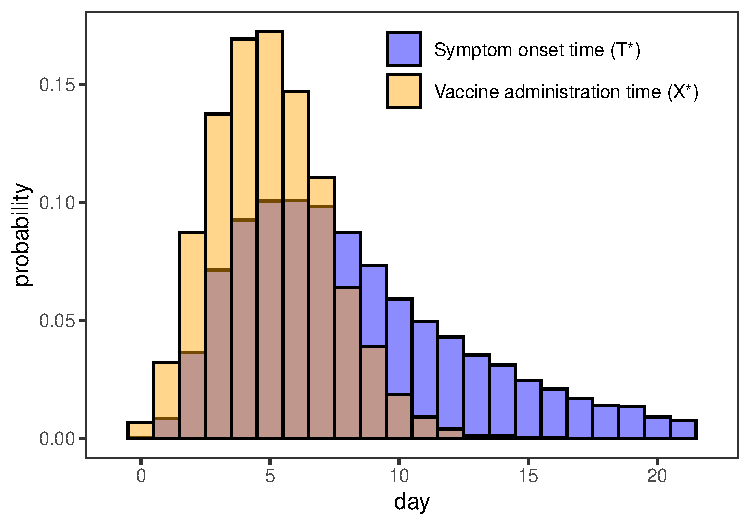
\includegraphics{../../../../3_figures/dist.pdf}
        \caption{Distribution of simulated vaccination times ($X^*$) among vaccinated and symptom onset times ($T^*$) among cases when $VE = 0$ over the 21 days of follow up showing the degree of overlap.}
        \label{fig:example_overlap_appendix}
    \end{figure}

    \clearpage 

    \begin{figure}[p]
        \centering
        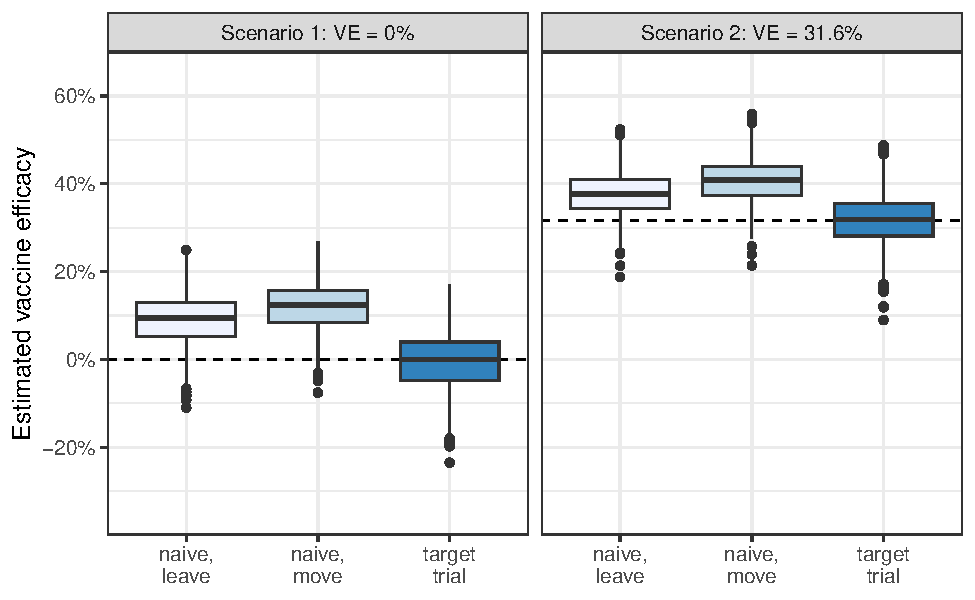
\includegraphics{../../../../3_figures/sim_rr.pdf}
        \caption{Simulated $VE$ estimates compared to the truth for the three estimation strategies described in section \ref{sec:simulation}. Based on 1000 monte carlo simulations. Dashed line shows true value in each scenario. \label{fig:sim_results_appendix}}
    \end{figure}

    \clearpage

    \begin{figure}[p]
        \centering
        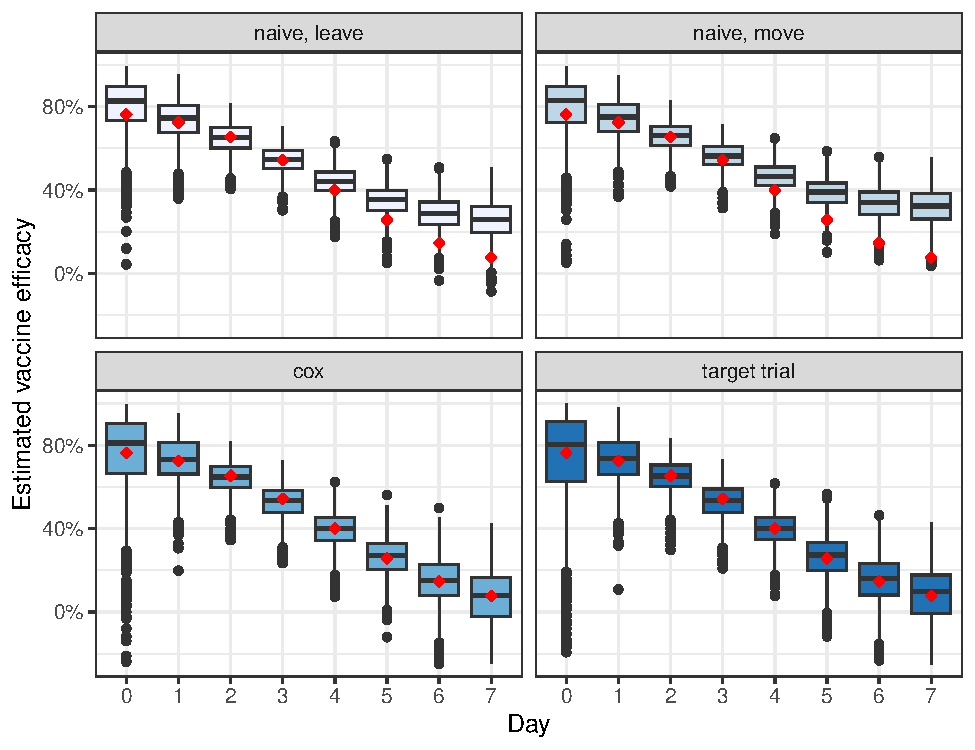
\includegraphics{../../../../3_figures/sim_hetx.pdf}
        \caption{Comparison of estimators under when vaccine effectiveness varies by postexposure administration time.\label{fig:sim_hetx}}
    \end{figure}

    \begin{figure}[p]
        \centering
        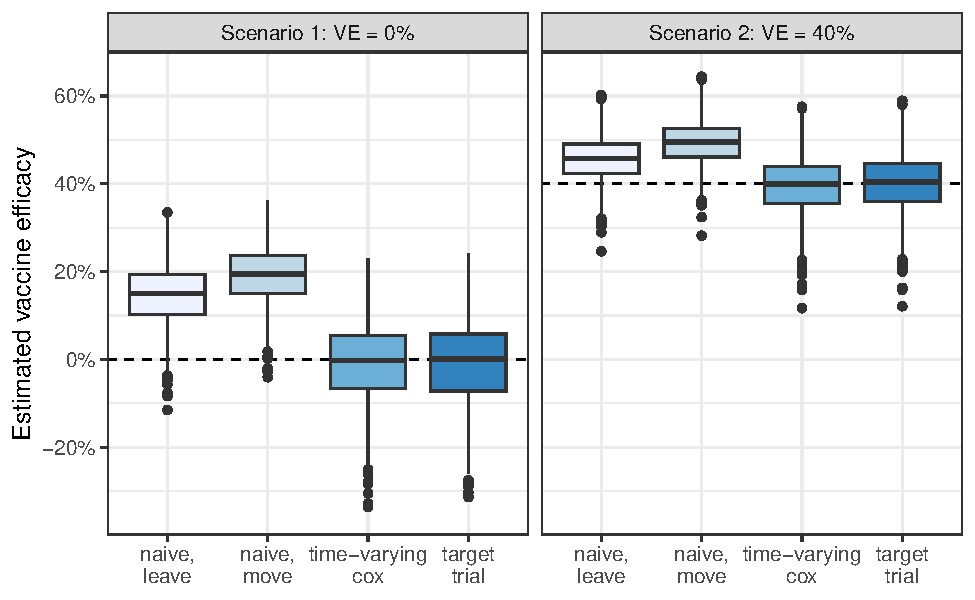
\includegraphics{../../../../3_figures/sim_hr.pdf}
        \caption{Comparison of estimators when calculating vaccine effectiveness using the hazard ratio instead of the risk ratio.\label{fig:sim_hr}}
    \end{figure}

    \begin{figure}[p]
        \centering
        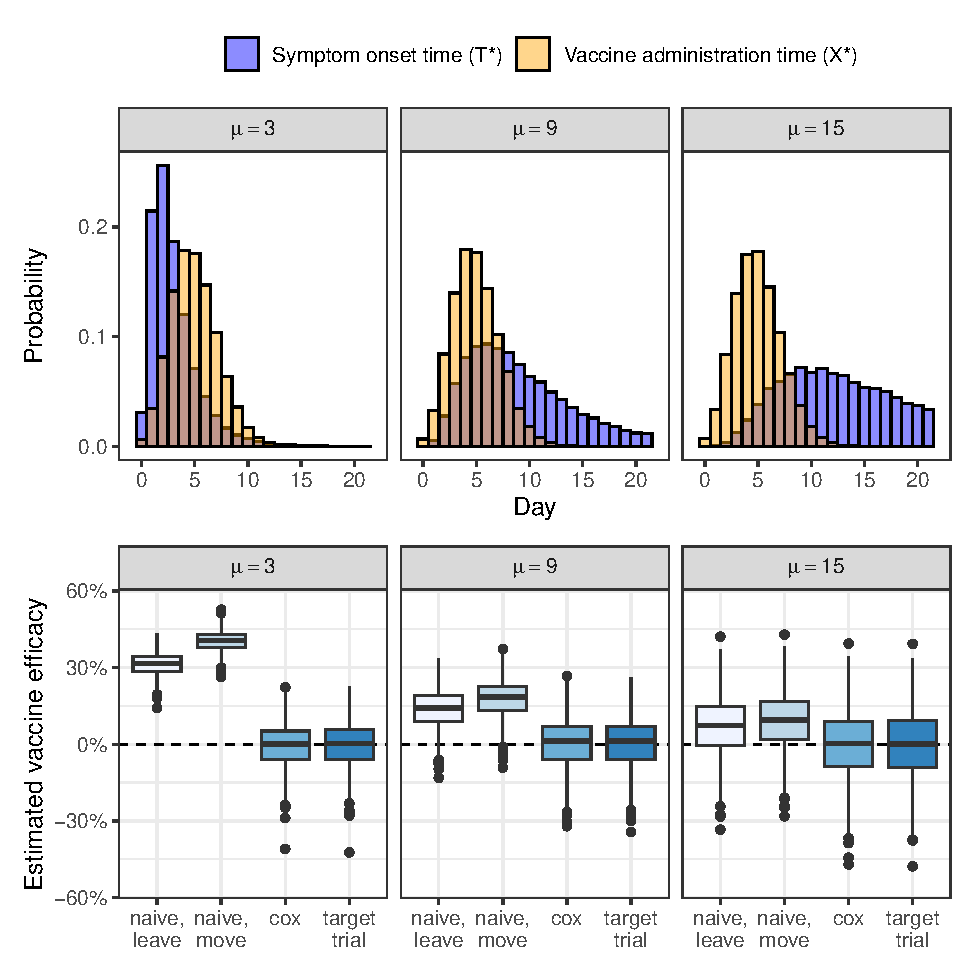
\includegraphics{../../../../3_figures/sim_overlap.pdf}
        \caption{Bias of na\"{i}ve methods varies with degree of overlap between vaccination delays and symptom onset times.\label{fig:sim_overlap}}
    \end{figure}

    \begin{figure}[p]
        \centering
        \includegraphics{../../../../3_figures/sim_TT.pdf}
        \caption{Simulated $VE$ estimates compared to the truth for four different target trial designs described in section \ref{sec:simulation}. Based on 1000 monte carlo simulations. Red dots shows true value in each scenario.\label{fig:sim_tt}}
    \end{figure}
    
    \clearpage
    

    \printbibliography[heading=subbibliography]
\end{refsection}
\end{appendices}